\section{Техническое задание}
\subsection{Основание для разработки}

Основанием для разработки является задание на выпускную квалификационную работу бакалавра "<Интеллектуальная система распознавания на основе изображений лица и отпечатков пальцев с интеграцией карт пропусков">.

\subsection{Цель и назначение разработки}

Интеллектуальная система предназначена для автоматизированного распознавания личности с использованием изображений лица, отпечатков пальцев и пропускных карт. Система разрабатывается для применения в задачах контроля доступа на охраняемые объекты, в учреждениях с ограниченным доступом, а также в корпоративной среде.

Система должна иметь возможность проведения идентификации посредством встроенного модуля биометрической аутентификации, без необходимости ввода паролей или взаимодействия с охранным персоналом.

Задачами данной разработки являются:
\begin{itemize}
\item реализация распознавания на основе изображений лица;
\item реализация распознавания на основе изображений отпечатков пальца;
\item интеграция карт пропуска;
\item реализация системы идентификации;
\end{itemize}

\subsection{Требования к программной системе}

\subsubsection{Требования к данным программной системы}


\subsubsection{Функциональные требования к интеллектуальной системе}

В разрабатываемой интеллектуальной системе должны
быть реализованы следующие функции: 
\begin{itemize}
    \item захват изображения лица с видеопотока;
\end{itemize}

На рисунке 2.1 предоставлены функциональные требования к системе,
представленные в виде диаграммы прецедентов.
\begin{figure}[H]
	\centering
	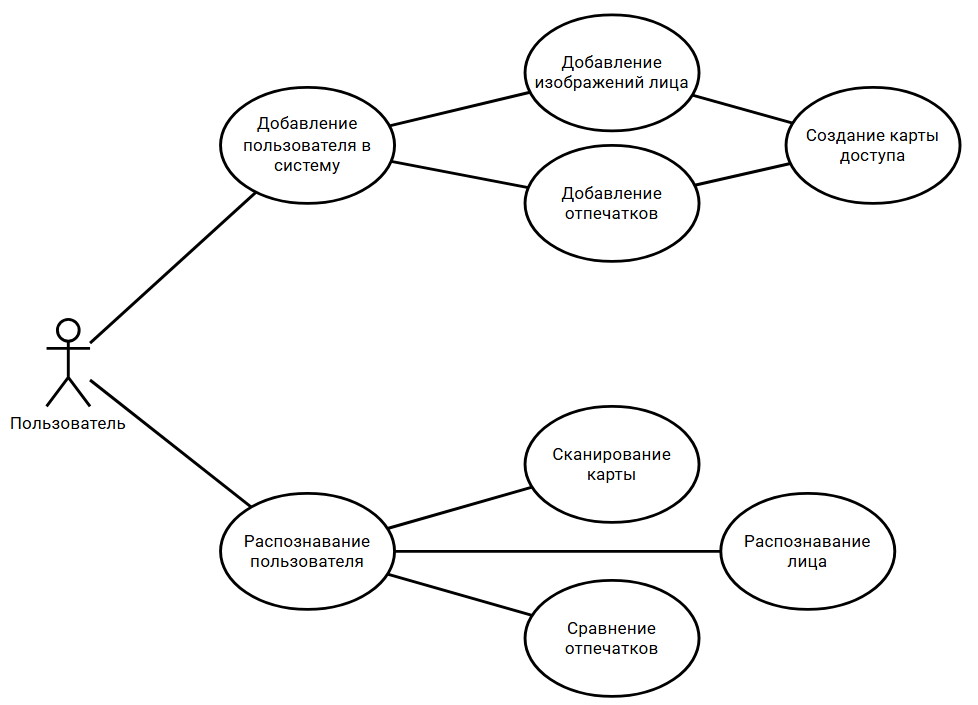
\includegraphics[width=1\linewidth]{images/UML}
	\caption{Диаграмма прецедентов}
	\label{fig:uml}
\end{figure}

\paragraph{Сценарий использования «Добавление изображений лица»}

Заинтересованные лица и их требования: пользователь желает добавить изображения лица в систему.

Предусловие: программа запущена, выбран режим «Добавить в систему».

Постусловие: программа сохраняет изображения лица пользователя  в систему.

Основной успешный сценарий:
\begin{enumerate}
	\item Пользователь нажимает на кнопку «Добавить в систему».
	\item Программа открывает диалоговое окно с указаниями для пользователя.
	\item Пользователь закрывает диалоговое окно.
	\item Программа запускает сканирования лица пользователя.
	\item Пользователь выполняет указания программы.
	\item Программа сохраняет изображения пользователя для дальнейшей обработки.
	\item Программа открывает диалоговое окно с результатом работы.
	\item Пользователь закрывает диалоговое окно и завершает сканирование лица.
\end{enumerate}

\paragraph{Сценарий использования «Добавление отпечатков»}

Заинтересованные лица и их требования: пользователь желает добавить изображения отпечатка в систему.

Предусловие: программа запущена, выбран режим «Добавить в систему», изображения лица добавлены.

Постусловие: программа сохраняет изображения отпечатка пользователя в систему.

Основной успешный сценарий:
\begin{enumerate}
	\item Пользователь нажимает на кнопку «Добавить в систему».
	\item Программа открывает диалоговое окно выбора файла.
	\item Пользователь выбирает файл в формате .jpg, содержащий изображение отпечатка пальца.
	\item Программа запускает обучение нейронной сети на основе изображения отпечатка.
	\item Программа сохраняет модель нейронной сети для дальнейшей работы.
\end{enumerate}

\paragraph{Сценарий использования «Создание карты доступа»}

Заинтересованные лица и их требования: пользователь желает создать карту для доступа в систему.

Предусловие: программа запущена, выбран режим «Добавить в систему», изображения лица и отпечатка добавлены.

Постусловие: программа создает карту доступа в систему.

Основной успешный сценарий:
\begin{enumerate}
	\item Пользователь нажимает на кнопку «Добавить в систему».
	\item Программа запускает создание карты доступа.
	\item Программа сохраняет карту доступа в систему.
\end{enumerate}

\paragraph{Сценарий использования «Сканирование карты»}

Заинтересованные лица и их требования: пользователь желает получить доступ в систему.

Предусловие: программа запущена, выбран режим «Распознавание пользователя».

Постусловие: программа переходит к распознаванию лица.

Основной успешный сценарий:
\begin{enumerate}
	\item Пользователь нажимает на кнопку «Распознавание пользователя».
	\item Программа открывает диалоговое окно с указаниями для пользователя.
	\item Пользователь закрывает диалоговое окно.
	\item Пользователь выполняет указания программы.
	\item Программа запускает сканирования карты пользователя.
	\item Программа получает данные с карты для дальнейшего распознавания.
\end{enumerate}

\paragraph{Сценарий использования «Распознавание лица»}

Заинтересованные лица и их требования: пользователь желает получить доступ в систему.

Предусловие: программа запущена, выбран режим «Распознавание пользователя», карта доступа распознана.

Постусловие: программа переходит к сравнению отпечатка.

Основной успешный сценарий:
\begin{enumerate}
	\item Пользователь нажимает на кнопку «Распознавание пользователя».
	\item Программа открывает диалоговое окно с указаниями для пользователя.
	\item Пользователь закрывает диалоговое окно.
	\item Пользователь выполняет указания программы.
	\item Программа запускает сканирования карты пользователя.
	\item Программа получает данные с карты для дальнейшего распознавания.
\end{enumerate}

\paragraph{Сценарий использования «Сравнение отпечатков»}

Заинтересованные лица и их требования: пользователь желает получить доступ в систему.

Предусловие: программа запущена, выбран режим «Распознавание пользователя», карта доступа и лицо распознаны.

Постусловие: программа выдает результат распознавания.

Основной успешный сценарий:
\begin{enumerate}
	\item Пользователь нажимает на кнопку «Распознавание пользователя».
	\item Программа открывает диалоговое окно с указаниями для пользователя.
	\item Пользователь закрывает диалоговое окно.
	\item Пользователь выполняет указания программы.
	\item Программа запускает сканирования карты пользователя.
	\item Программа получает данные с карты для дальнейшего распознавания.
\end{enumerate}


\subsubsection{Требования пользователя к интерфейсу приложения}

 Приложение должно иметь следующие экраны:
 
 \begin{enumerate}
 	\item Экран «Идентификация». Основной экран, реализующий
 	функционал распознавания пользователя на основе изображений лица и отпечатка пальца.
 	\item Экран «Добавление в систему». Экран, позволяющий добавлять пользователя в систему, путём сохранения изображений лица и отпечатков пальца с генерацией карты доступа.
 \end{enumerate}


\subsubsection{Нефункциональные требования к программной системе}

\paragraph {Требования к надежности}

Программная система должна обеспечивать стабильную работу в различных условиях эксплуатации. В процессе работы приложения могут возникнуть следующие аварийные ситуации:
\begin{enumerate}
	\item отсутствие подключения к камере для получения изображений;
	\item ошибка доступа к файлам изображения;
\end{enumerate}

Для предотвращения аварийных ситуаций программа должна корректно обрабатывать исключения при работе с файлами, предоставляя пользователям информативные сообщения об ошибках. В случае проблем с отсутствием прав доступа к директории сохранения файлов, полученных в результате работы программы, программа должна открывать диалоговое окно с выбором другой директории.

\paragraph {Требования к программному обеспечению}



\paragraph {Требования к аппаратному обеспечению}



\subsection{Требования к оформлению документации}

Разработка программной документации и программного изделия должна производиться согласно ГОСТ 19.102-77 и ГОСТ 34.601-90. Единая система программной документации.

Программная документация должна включать в себя:
\begin{itemize}
	\item анализ предметной области;
	\item техническое задания;
	\item технический проект;
	\item рабочий проект.
\end{itemize}